\documentclass[10pt,twocolumn,letterpaper]{article}

\usepackage{cvpr}
\usepackage{times}
\usepackage{epsfig}
\usepackage{graphicx}
\usepackage{amsmath}
\usepackage{amssymb}
\usepackage{algorithm,algorithmic}

\newcommand{\highlight}[1]{{\color{red}#1}}
% Include other packages here, before hyperref.

% If you comment hyperref and then uncomment it, you should delete
% egpaper.aux before re-running latex.  (Or just hit 'q' on the first latex
% run, let it finish, and you should be clear).
\usepackage[breaklinks=true,bookmarks=false]{hyperref}

\cvprfinalcopy % *** Uncomment this line for the final submission

\def\cvprPaperID{****} % *** Enter the CVPR Paper ID here
\def\httilde{\mbox{\tt\raisebox{-.5ex}{\symbol{126}}}}

% Pages are numbered in submission mode, and unnumbered in camera-ready
%\ifcvprfinal\pagestyle{empty}\fi
\setcounter{page}{1}
\begin{document}

%%%%%%%%% TITLE
\title{Deep Reinforcement Learning for Atari Games}

\author{Liyang Xie \and Xiao Zeng \and Kaixiang Lin\\}
% For a paper whose authors are all at the same institution,
% omit the following lines up until the closing ``}''.
% Additional authors and addresses can be added with ``\and'',
% just like the second author.
% To save space, use either the email address or home page, not both
% \and
% Second Author\\
% Institution2\\
% First line of institution2 address\\
% {\tt\small secondauthor@i2.org}}

\maketitle
%\thispagestyle{empty}


%%%%%%%%% ABSTRACT
\begin{abstract}
%!TEX root = main.tex 
Deep reinforcement learning (DRL) has achieved
unprecedented success in many challenging
domains~\cite{mnih2015human,silver2016mastering}, by combining the power of modeling complex
functions of deep learning and the fairly general-purpose framework of reinforcement learning.
In this project, we \textbf{propose} a new methods that firstly distill the knowledge to a dueling Q-network,
by which the training procedure can be speed up.
Also, we \textbf{implemented} another state-of-arts method--A3C algorithm~\cite{mnih2016asynchronous} as our
baseline.
The extensive experiments have been conducted on OpenAI Gym~\cite{brockman2016openai} to evaluate 
our proposed method and implementations.
% competing state-of-arts such as A3C algorithm~\cite{mnih2016asynchronous}. 
\end{abstract}

%%%%%%%%% BODY TEXT
\section{Introduction}
%!TEX root = main.tex


Deep reinforcement learning has been attracted widely interests from both
industry and academia. The reason is that the combination of deep learning and
reinforcement learning has shown the effectiveness on lots of applications
and more supursingly, the good performances can be achieved without problem-
specific engineering.






OpenAI Gym~\cite{brockman2016openai} is a toolkit for reinforcement learning research. 


%-------------------------------------------------------------------------

\section{Related Work}
%!TEX root = main.tex

The milestone of the deep reinforcement learning is deep Q-learning(DQN)\cite{mnih2013playing}, a variant of Q-learning, proposed by DeepMind. It is the first deep learning model trying to learn control policies with reinforcement learning. In 2015, DeepMind presented an improved version of DQN\cite{mnih2015human}. Their work outperformed previous algorithms and achieved a capability comparable to that of professional human-being.
%

while DQN performs well in fully-observable environments, it achieves poor result in partially observable environments. To address this problem, Hausknecht and Stone\textit{ et al.} \cite{hausknecht2015deep} introduced the Deep Recurrent Q-Networks(DRQN). The idea is to build a recurrent neural network such as LSTM on top of the DQN model.
%

One drawback of DQN is that it needs to aggregate over time to overcome data non-stationarity. To reduce the overhead caused by experience replay, DeepMind \cite{mnih2016asynchronous} proposed a another paradigm for deep reinforcement learning: multiple agents are running in parallel asynchronously on multiple instances of the environment. Using the paradigm makes Q-learning both efficient and compatible with deep neural network at the same time. They named their best method \textit{asynchronous advantage actor-critic} (A3C). Experiments showed that A3C not only achieved better result but also required less computational cost.
%
More recently, AlphaGo\cite{brockman2016openai}, which is also developed by DeepMind, defeated Lee Sedol and became the first 'Artificial Intelligence' who beated 9-dan professional human Go player. Behind the AlphaGo is deep neutral network integrated with reinforcement learning improving the play strategy.
%
One drawback of DQN is that it needs to aggregate over time to overcome data non-stationarity. To reduce the overhead caused by experience replay, DeepMind \cite{mnih2016asynchronous} proposed a very different paradigm for deep reinforcement learning: multiple agents are running in parallel asynchronously on multiple instances of the environment. Using the paradigm makes Q-learning both efficient and compatible with deep neural network at the same time. They named their best method \textit{asynchronous advantage actor-critic} (A3C). Experiments showed that A3C not only achieved better result but also required less computational cost.
%
RDQN sometimes learn unrealistically high action values because it includes a maximization step over estimated action values, which tends to
prefer overestimated to underestimated values. This has been demonstrated in some games in the Atari 2600 domain. The idea of double Q-learning algorithm \cite{van2015deep} not only yields more accurate value estimates, but leads to much higher scores on several games. This demonstrates that the overestimations of DQN indeed lead to poorer policies and that it is beneficial to reduce them.

Other application of reinforcement Learning in designing game includes linear evaluation function-based learning of local shape in the game of Go \cite{silver2007reinforcement} and learning control policies for text-based games \cite{narasimhan2015language}


%-------------------------------------------------------------------------

\section{Methodology}
%!TEX root = main.tex
% \subsection{Deep Reinforcement Learning}
% In this project, we plan to develop and implement a novel deep reinforcement learning algorithm and compete with other methods on OpenAI Gym. Specifically, we will implement DQN and use it as baseline. Based on its performance, we will conduct a series of analysis and try to improve the baseline.
%
Deep Q-Networks (DQN) adopts a neural network parametrized by $\theta$. The goal is to obtain an optimal estimate of the Q-function by training a model parameterized by $\theta$:
\begin{equation*}
\theta = \arg\max_\theta Q(s,a;\theta)
\end{equation*}
where $s$ stands for a state and $a$ denotes the corresponding action.
There are basically two ways to update $\theta$ in reinforcement learning. The first one is value-based Q-learning where $\theta$ is learned by minimizing a loss function;
$$
L_{i}(\theta_{i}) = \mathbb{E}(r+\gamma \max_{a'}Q(s',a';\theta_{i-1})-Q(s,a;\theta_{i})))^2 
$$
where $s'$ is the state after $s$ and $a'$ is the action in state $s'$
The second algorithm is known as Sarsa where the Q-function is updated by minimizing the following loss function:
$$
L_{i}(\theta_{i}) = \mathbb{E}(r+\gamma Q(s',a';\theta_{i-1})-Q(s,a;\theta_{i})))^2 
$$

Empirically, the above mentioned algorithms are usually not able to converge
during updating. There are many reasons lead to this: 1) One-Step Update. They
only consider one step when computing the loss. Using one step leads to slow
convergence because many update steps are required to affect the relevant sate
action pairs. To overcome this, we can use n-step rewards when updating
$\theta$. 2) Data Sequences Correlation. The training data is sequential and
successive data are correlated which may make the optimization fall into local
optima. Experience replay is adopted to break the correlations between
successive updates. 3) Varying Target. The target is highly correlated with
predicted Q-values and produces oscillation during training. Instead, a
technique which fixes the targets for several thousand updates is employed to
reduce the correlations.


%!TEX root = main.tex

In this project, we plan to develop and implement a novel deep reinforcement learning algorithm and compete with other methods on OpenAI Gym. Specifically, we will implement DQN and use it as baseline. Based on its performance, we will conduct a series of analysis and try to improve the baseline.
%
DQN adopts a neural network parametrized by $\theta$. The goal is to obtain an optimal estimate of the Q-function by training a model:
\begin{equation*}
\theta = \arg\max_\theta Q(s,a;\theta)
\end{equation*}
where $s$ stands for a state and $a$ denotes the corresponding action. 
The evaluation will be performed on the OpenAI Gym.

The algorithm we used here to beat the baseline is the asynchronous advantage actor-critic (A3C) algorithm that proposed by Volodymyr et al.~\cite{mnih2016asynchronous}. It is a value-based model-free reinforcement learning method. This algorithm maintains a policy $\pi (a_{t}|s_{t};\theta)$ and the estimation of the value function $V(s_{t};\theta_{v})$, where $\theta$ and $\theta_{v}$ are the parameter. These two parameters are learned by the take the gradient of $\log \pi (a_{t}|s_{t};\theta) A(s_{t},a_{t};\theta,\theta_{v})$ with respect to $\theta^{\prime}$. The update of $\pi (a_{t}|s_{t};\theta)$ and $V(s_{t};\theta_{v})$ happens either after every $t_{max}$ actions or when a terminal state is reached. Combine with the idea in deep learning, here we use a convolutional neural network that has one softmax output for the policy $\pi (a_{t}|s_{t};\theta)$ and and
one linear output for the value function $V(s_{t};\theta_{v})$. The algorithm is shown below for completeness.


%-------------------------------------------------------------------------

\section{Experiments}
%!TEX root = main.tex


In this section, we empirically evaluate the effectiveness and the efficiency of the
state-of-arts in deep reinforcement learing on OpenAI gym Atari environment. Note 
that at current stage, we didn't propose any new methods in deep reinforcement learning;
instead our first stage is to learning the most advanced algorithms first using public
available online resources. 


\subsection{Environments}

In order to evaluate the algorithm, we conduct our experiments on Atari environment
provided by OpenAI. The description of Atari environment is as follows:
\begin{quote}
Maximize your score in the Atari 2600 game. In this
environment, the observation is an RGB image of the screen, which is an array
of shape (210, 160, 3) Each action is repeatedly performed for a duration of
kk frames, where kk is uniformly sampled from \{2, 3, 4\}~\cite{brockman2016openai}
\end{quote}

We choose three Atari games as our testing environment, all of which are unsolved environments, 
which means those games don't have a specific reward that you can consider it as the end of game:

\begin{enumerate}
\item Breakout-v0\\
In this game, player control a paddles at the bottom of screen and try to bounce the ball upwards
to hit those bricks as soon and as much as possible, as illustrated in Fig~\ref{fig:A3C_baselines} (a). 

\item Pong-v0\\
In this game, players control a paddles at the right of screen and try to bounce the ball pass the
other player at the left of screen, as illustrated in Fig~\ref{fig:A3C_baselines} (b). 

\item Phoenix-v0
In this game, players control a spaceship by moving it horizontally at the bottom of screen, as 
illustrated in Fig~\ref{fig:A3C_baselines} (c), trying to destroy the enemies by firing upwards 
and avoiding the attack from those enemies. 
\end{enumerate}

\subsection{Baselines}

In this section, we introduce the implementation details of the baselines we used.

% As we introduced in Methodology section, we use two neural network to model policy function
% and value function, respectively. 
The structure of policy network is shown as in Table.\ref{table.cnn_detail}:

\begin{table}[!ht]
	\centering
	\caption{CNN detail}
	\label{table.cnn_detail}
	\begin{tabular}{c|c|c|c}
		\textbf{Type} & \textbf{size} & \textbf{\# filters} & \textbf{activation} \\ \hline
		convolution & $5\times5$ & 32 & Relu \\ 
		max pooling & $2\times2$ &  &  \\
		convolution & $5\times5$ & 32 & Relu \\
		max pooling & $2\times2$ &  &  \\
		convolution & $4\times4$ & 64 & Relu \\
		max pooling & $2\times2$ &  &  \\
		convolution & $3\times3$ & 64 & Relu \\
		fully connected & 512 &  & PRelu \\
		softmax &  &  & 
	\end{tabular}
\end{table}
%\begin{enumerate}
%\item Convolution layer: $(5 \times 5, 32)$ 
%\item Maximum pooling layer: $(2 \times 2) $
%\item Convolution layer: $(5 \times 5, 32)$ 
%\item Maximum pooling layer: $(2 \times 2) $
%\item Convolution layer: $(4 \times 4, 64)$ 
%\item Maximum pooling layer: $(2 \times 2) $
%\item Convolution layer: $(3 \times 3, 64)$ 
%\item Fully connected layer with 512 nodes and PReLU activation function.
%\item Softmax layer to predict the probability over all possible actions.
%\end{enumerate}
We modified the implementation of A3C from \href{https://github.com/ppwwyyxx/tensorpack}{tensorpack} repository.


\subsection{experimental results}




\subsubsection{Policy Gradient}
%!TEX root = main.tex

The results of policy gradient method on CartPole environment is show
in Figure~\ref{fig:pg_cartpole}. Also, a video illustration can be found
in \href{https://gym.openai.com/evaluations/eval_UaXIaMm1QxPGgW45KHtTA#reproducibility}{this link}.
As we can see in both the video and the figure, the game was solved by 
few hundred episodes. This show the effectiveness of policy gradient methods
and we further train a this model in a more complex environment. 

\begin{figure}[h!]
\centering
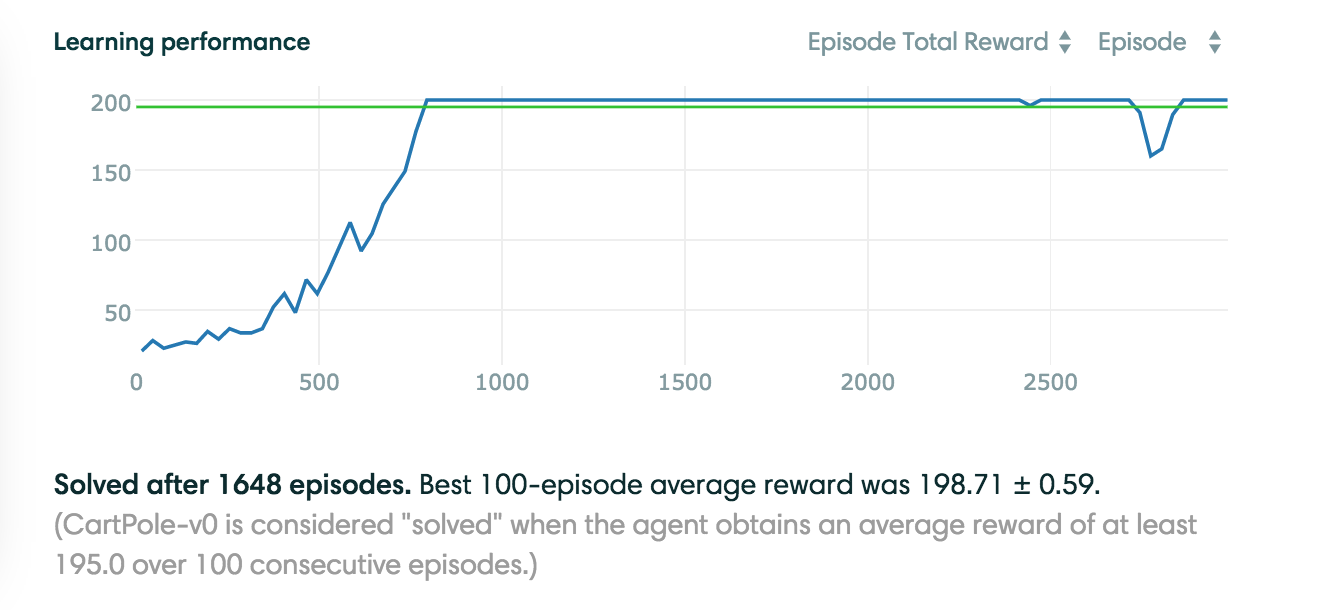
\includegraphics[width=0.49\textwidth]{./fig/pg_cartpole.png} 
\caption{The plot of reward for cartpole game. The x-axis is the number
of episodes it has been trained. The y-axis is the cumulative reward in 
per episode. The higher the better. }
\label{fig:pg_cartpole}
\end{figure}


The performance on Pong game is plot in Figure~\ref{fig:pg_pong} and a video
illustration can be found \href{https://gym.openai.com/evaluations/eval_dODFoXO2S4y5TuUZMX7Nw}{at this link}. As it
shown in the figure, this game requires more than 10000 episodes to get 
a model better than the baseline provided by OpenAI gym. It much more complicated
than the CartPole, since the state and action space is more complex than 
that. The structure of this policy is a single hidden layer with eight
hidden nodes fully connected network and it works. It may perform
better if we use a convolutional network to replace this one, but compared 
the results in dueling DQN, it seems the algorithms of reinforcement learning
itself is more important, other than the specific network architecture. 

\begin{figure}[h!]
\centering
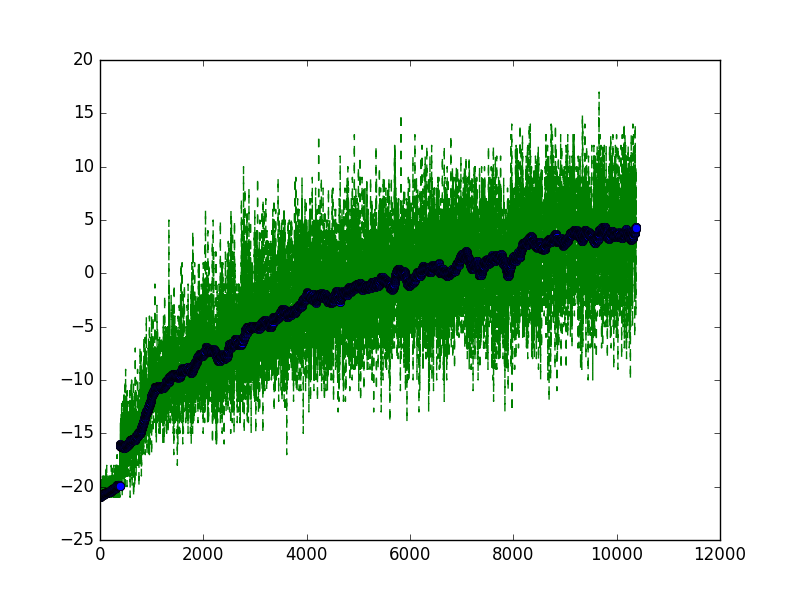
\includegraphics[width=0.49\textwidth]{./fig/pg_pong_rewardsplot.png} 
\caption{The plot of reward for pong game. The x-axis is the number
of episodes it has been trained. The y-axis is the cumulative reward in 
per episode. The higher the better. }
\label{fig:pg_pong}
\end{figure}




\subsubsection{Asynchronous advantage actor-critic}
The experimental results are illustrated in the Fig~\ref{fig:A3C_baselines}. Please also
see the video animation by clicking the captions under each figures. 
% The results are acquired by a pre-trained model and then follow the A3C models,

\begin{figure}[h!]
\centering
\begin{tabular}{c}
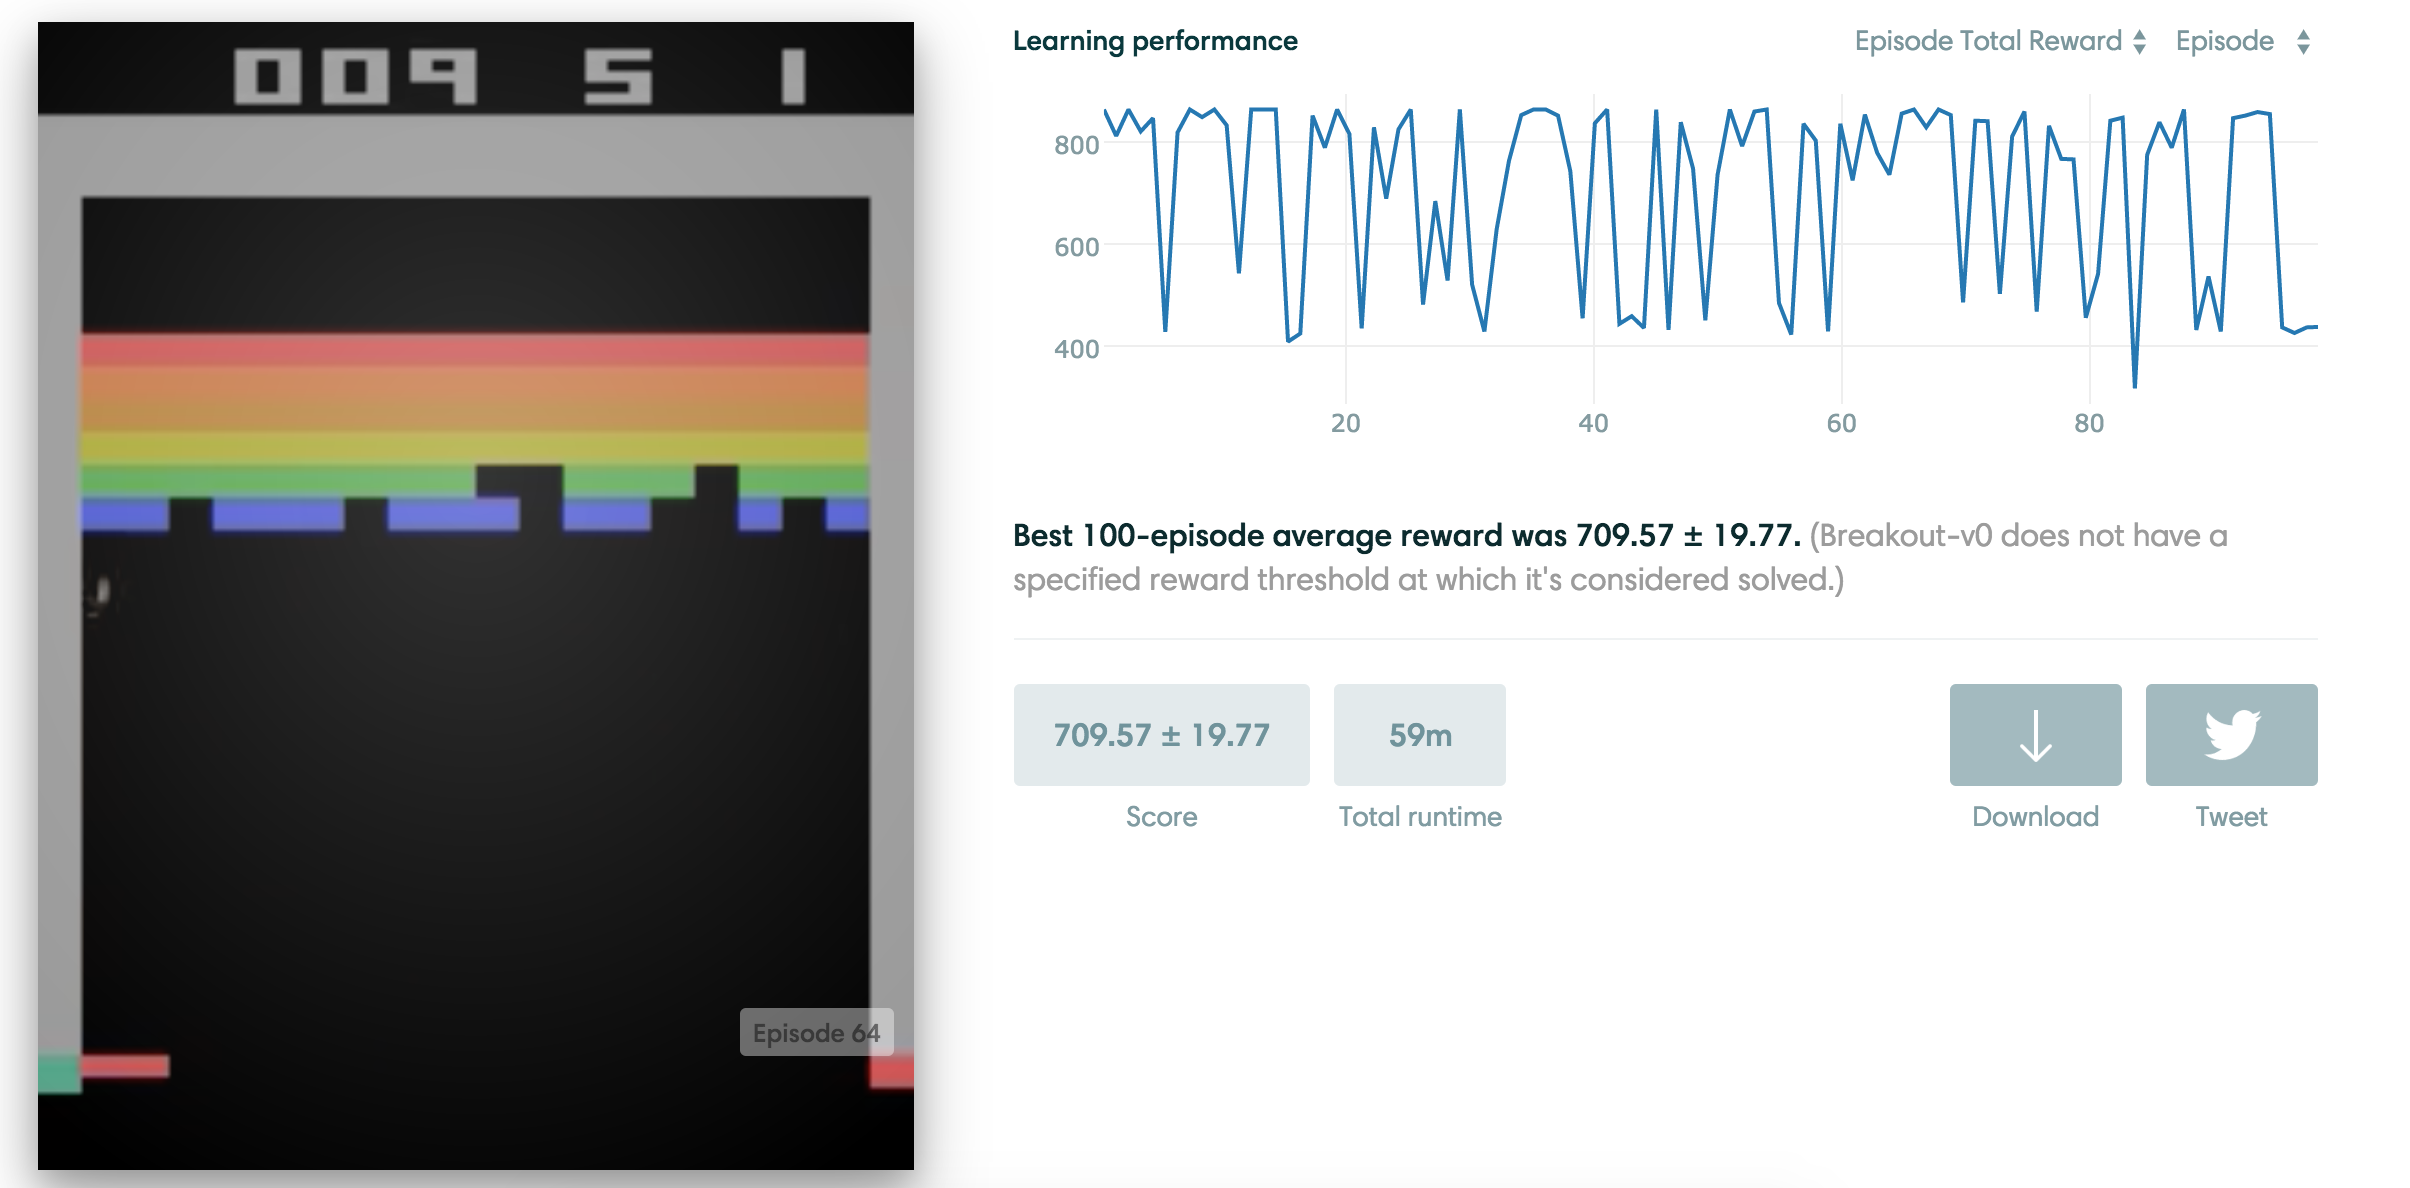
\includegraphics[width=0.49\textwidth]{./fig/A3C_Breakout-v0.png} \\
(a) \href{https://gym.openai.com/evaluations/eval_i9E40nAQuOTiSa0bxYBA#reproducibility}{Breakout-v0} \\
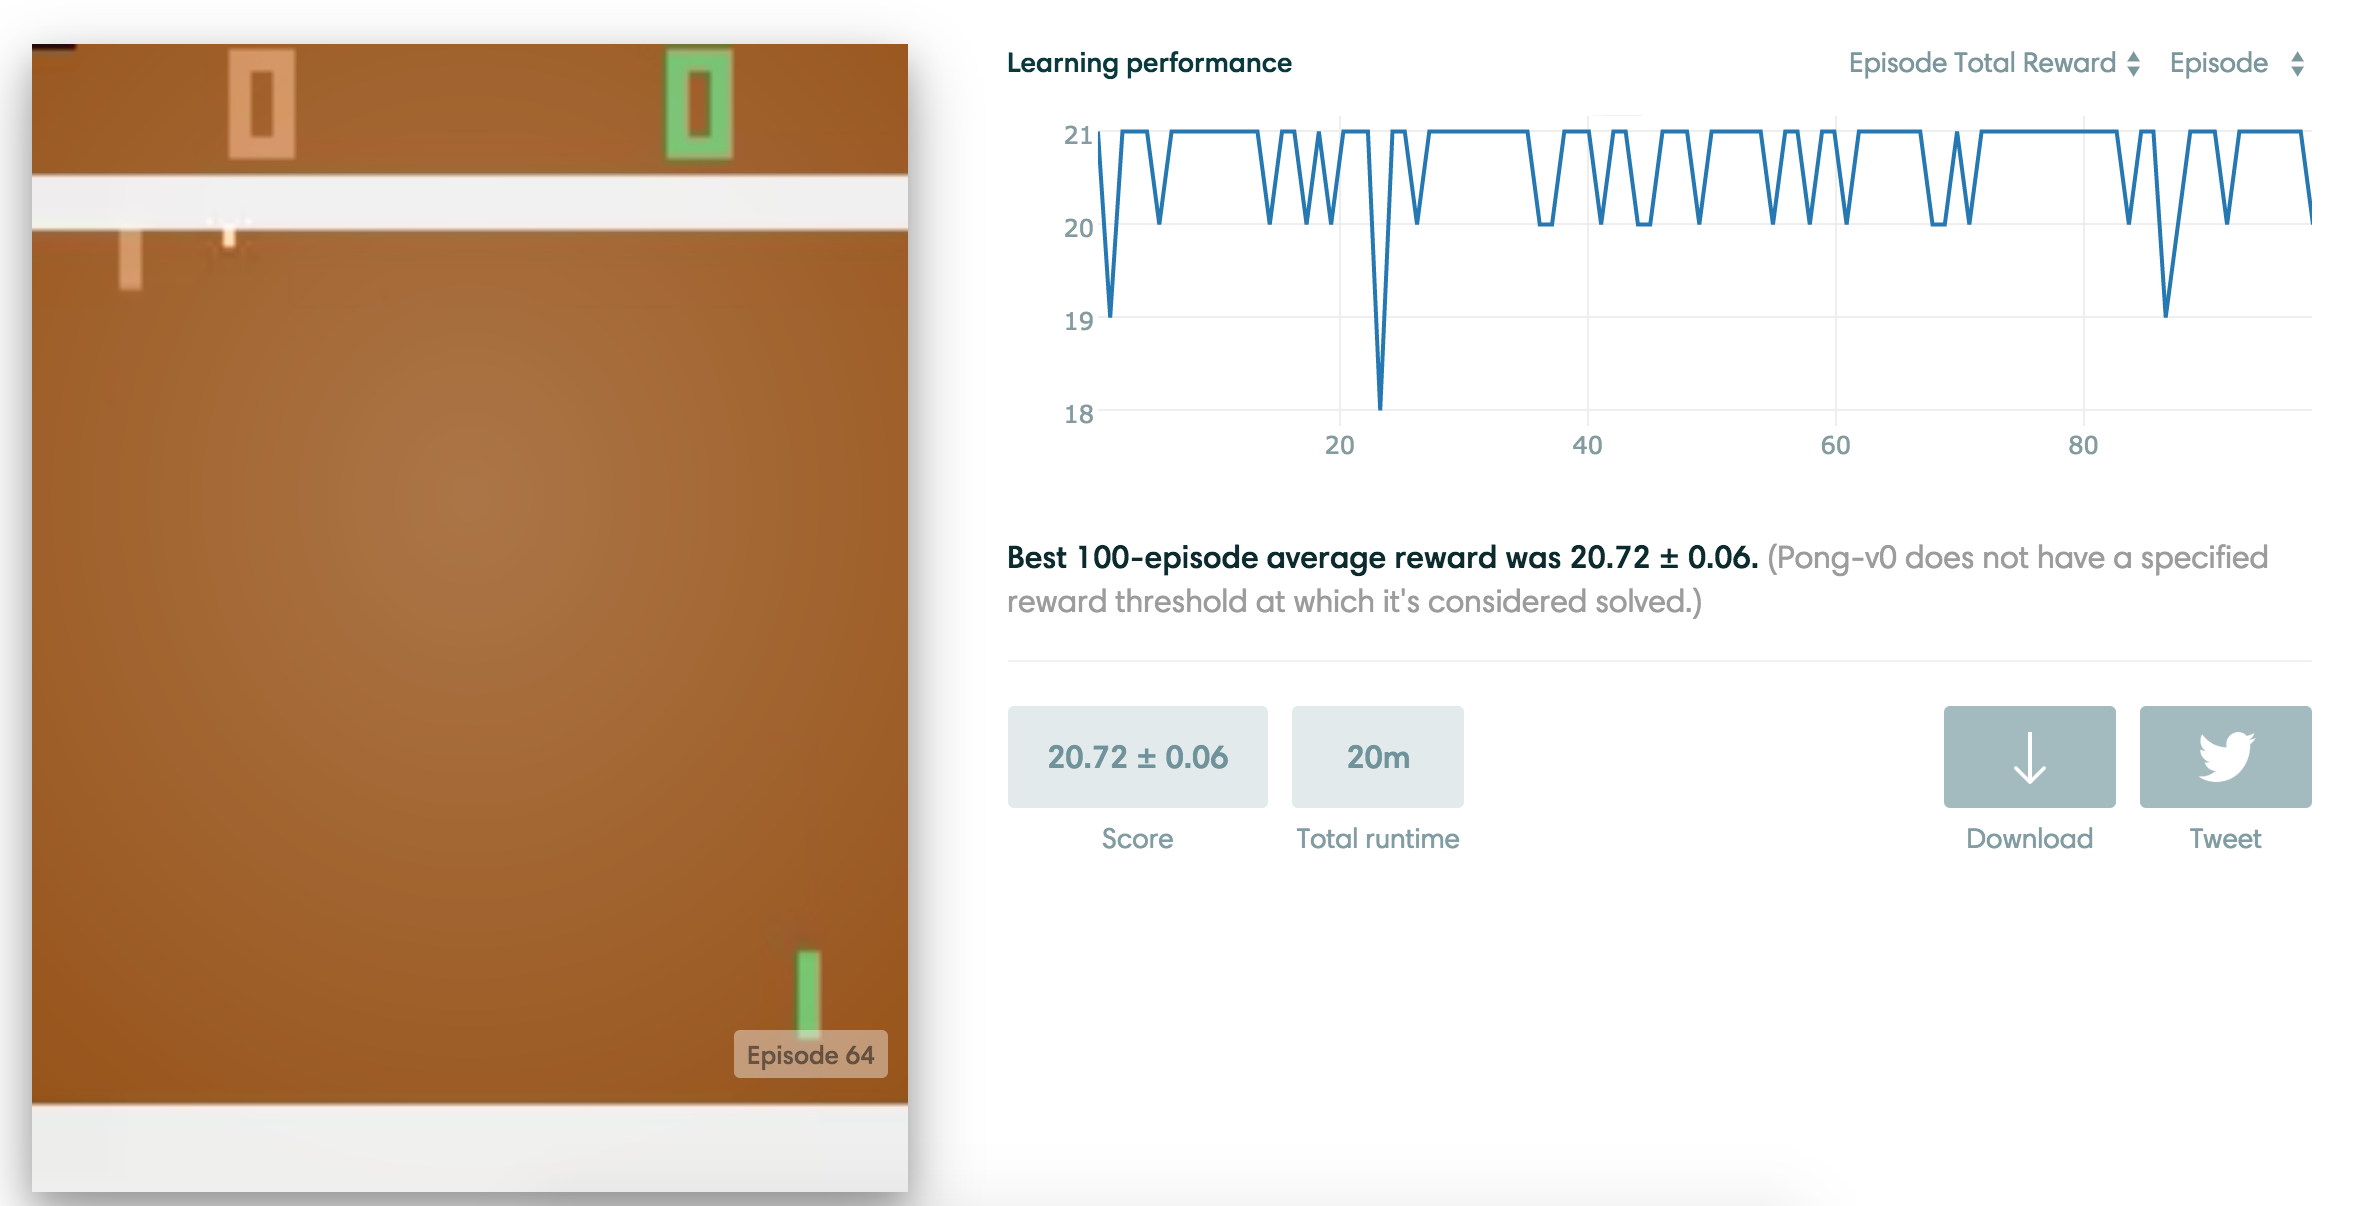
\includegraphics[width=0.49\textwidth]{./fig/A3C_Pong-v0.png} \\
(b) \href{https://gym.openai.com/evaluations/eval_mvXuxP13SSacO01UIhsg#reproducibility}{Pong-v0} \\
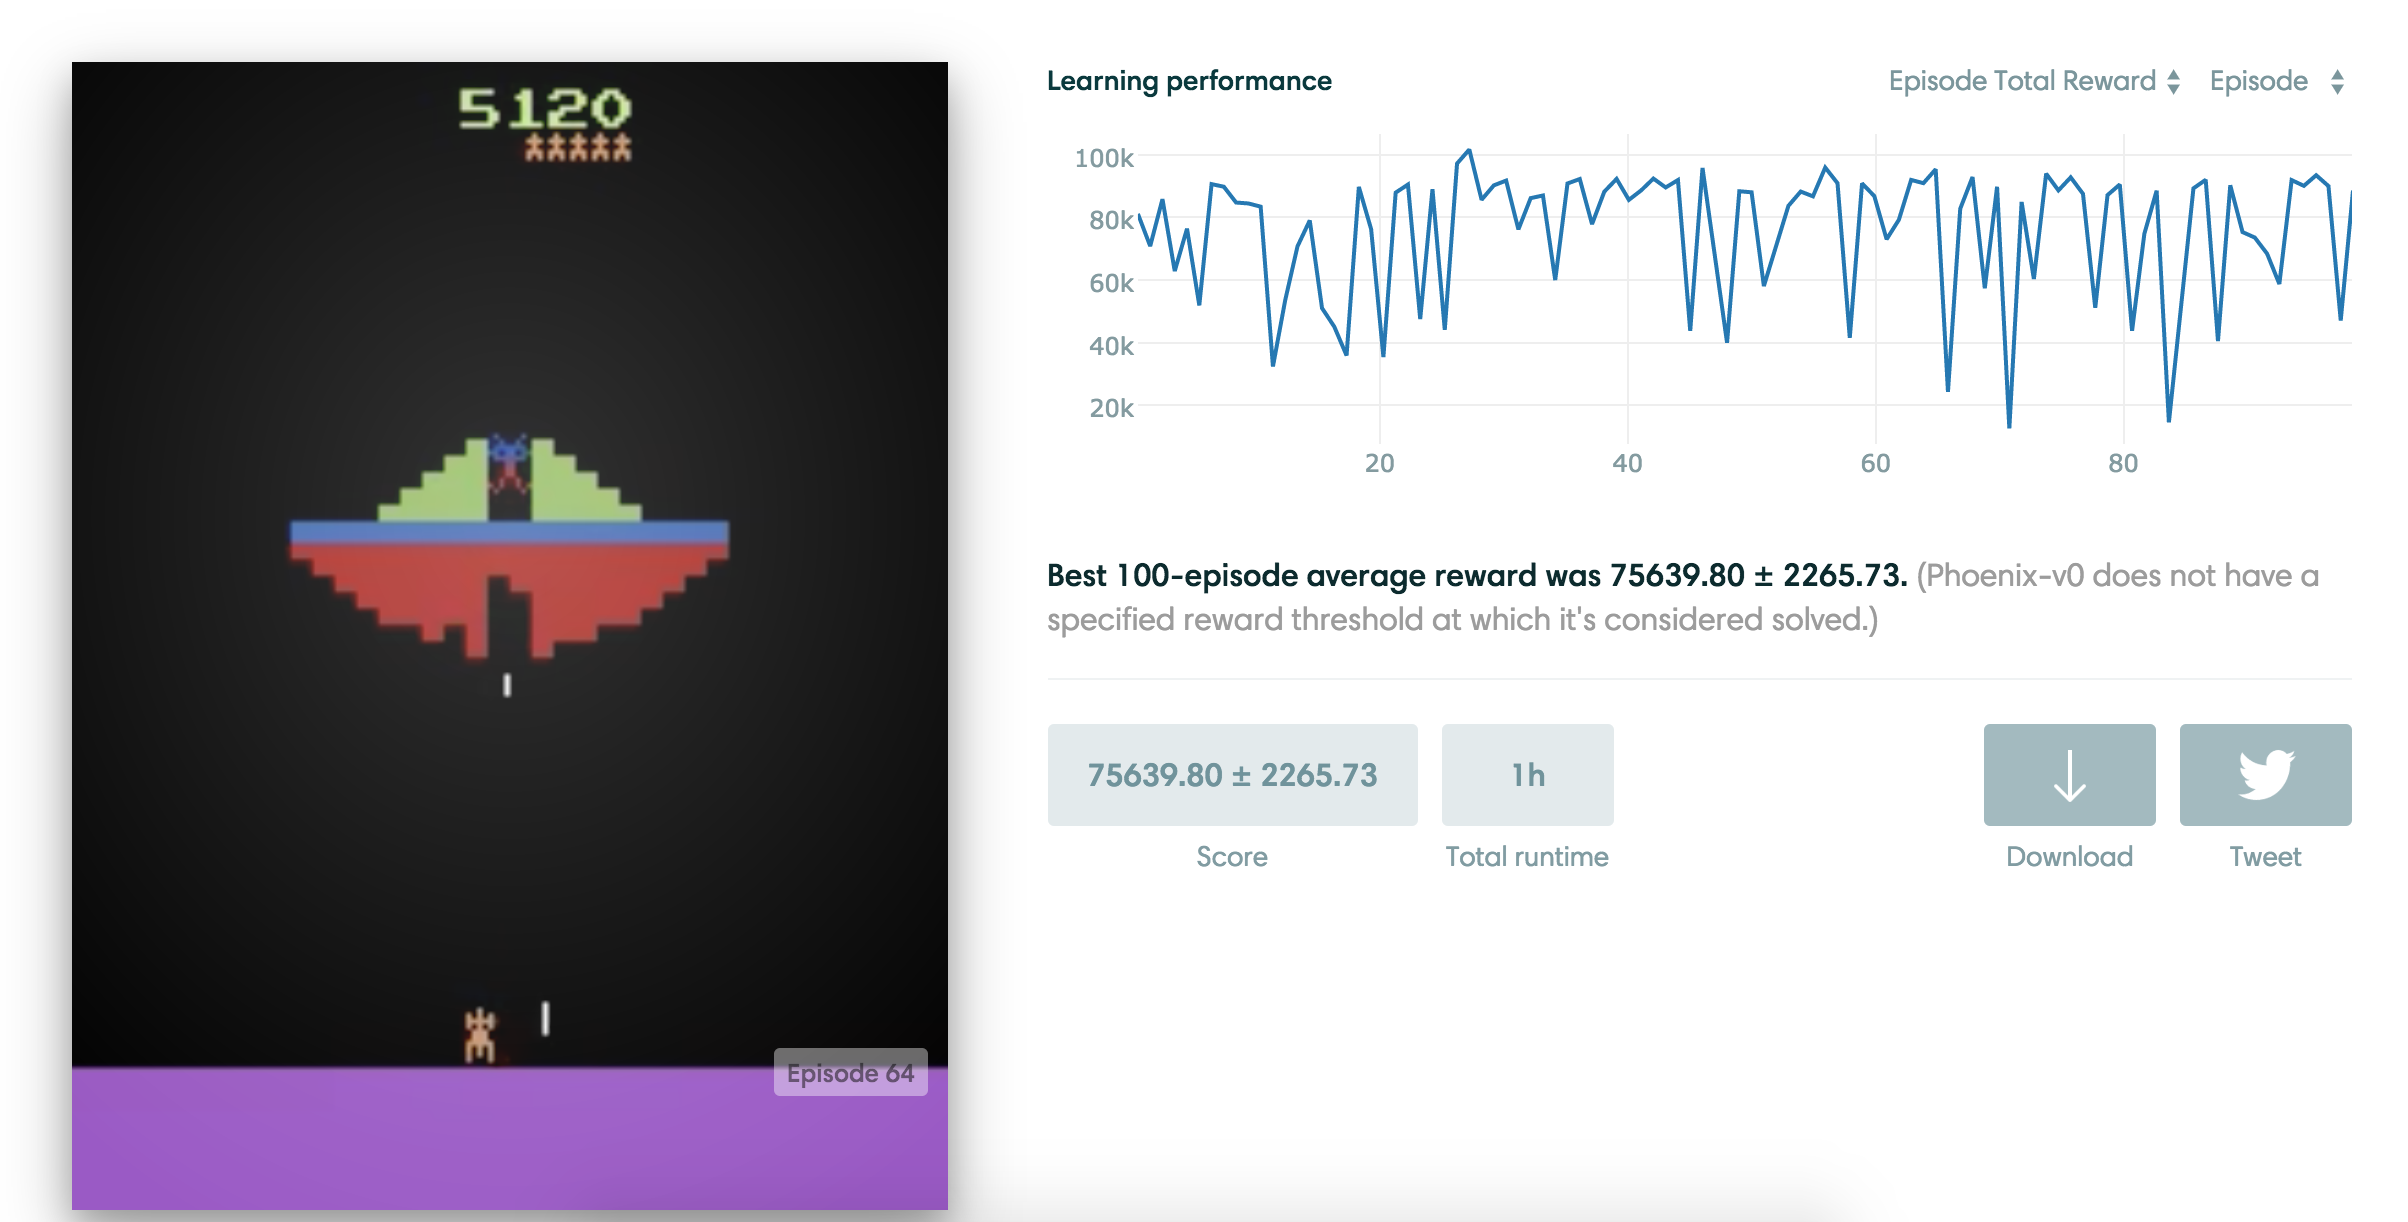
\includegraphics[width=0.49\textwidth]{./fig/A3C_Phoenix-v0.png} \\
(c) \href{https://gym.openai.com/evaluations/eval_Gva8XrEvTQi63KOd5Gyq1Q#reproducibility}{Phoenix-v0} \\
\end{tabular}
\caption{The results of 100 epsiodes on three environments by applying A3C algorithms. By clicking the name of each environment 
beneath the figures, you will see the video for each game played by trained agent.}
\label{fig:A3C_baselines}
\end{figure}





\section{Dueling Q-Network}
%!TEX root = main.tex
\subsection{From Single to Dueling}
To generalize learning across actions without imposing any change to the underlying reinforcement learning algorithm, Ziyu Wang \textit{et al.}\cite{wang2015dueling} proposed dueling Q-network.

\begin{figure}[ht!]
	\centering
	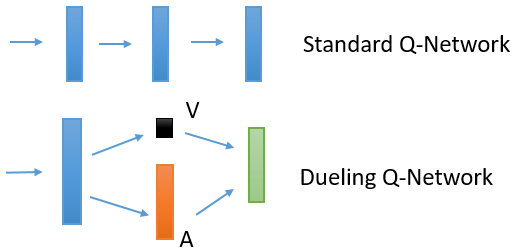
\includegraphics[width=0.49\textwidth]{./fig/dueling.png} \\
	\caption{The architecture of Dueling Q-Network.}
	\label{fig:dueling_q_network}
\end{figure}

As shown in Fig.\ref{fig:dueling_q_network}, The top one is standard Q-network which has only one stream. 
%
The dueling network has two-streams in the middle. One is called $V value$, which denotes how good it is to be in the current state. The other is called $Advantage$, which represents how good is every action.
%
As a result, the dueling Q-network can learn which states are valuable, without having to learn the effect of each action for each state. 

\subsection{Experience Replay}

During sampling, we adopt \textit{experience replay}\cite{adam2012experience} in order to stabilizing the training process.
%
The basic idea is that through keeping an agent’s experiences , we can randomly sample experiences from memory and breaks the time correlation of the data.
%
Specifically, by keeping the experiences, the Q-network can avoid learning about what it is immediately doing in the environment, and it can learn from the past experiences. 
%
These experiences are stored as tuples of \textit{(state,action,reward,next state)} and updated online. (As new experiences come in, old ones are removed randomly). 
%
When optimizing, we simply sample a uniform batch of random experiences from memory, and train our network with them.
%
As shown in Fig.\ref{fig:experience_replay}, we first sample the experiences from environment randomly, which means for every given state $s$, we take a random action $a$ and record the new state $s'$ and new reward $r'$.

\begin{figure}[ht!]
	\centering
	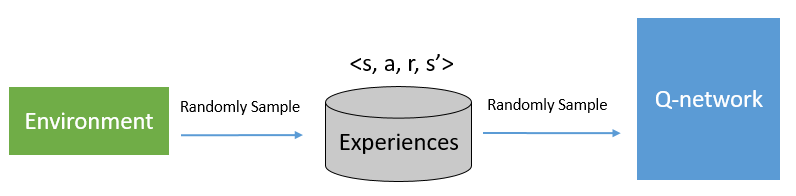
\includegraphics[width=0.49\textwidth]{./fig/experience_replay.png} \\
	\caption{Illustration of experience replay.}
	\label{fig:experience_replay}
\end{figure}

\subsection{Target Network}
To reduce the oscillation during training, we employ Target Network Strategy\cite{lillicrap2015continuous}.
%
Specifically, at every step of training, the target Q-values are shifting if we use the same network to produce target Q-values.
%
If we are using a constantly shifting target Q-values to optimize our Q-network, the updates can easily run out of control and fall in local optima. The estimates of Q-values will then be inaccurate.
%
The idea behind target network is that it utilizes a second network called target network which has exactly the same architecture as original one during the training procedure.
%
The target network is used to generate the target Q values. The target Q-values are used to compute the loss during training.
%
In order to mitigate that risk, the target network’s weights are fixed for a number of iterations, and periodically or updated to the original Q-networks values. 
%
we can achieve more stable training procedure if target network strategy is used.




\section{Transfering Knowledge}
%!TEX root = main.tex
In this section, we are interested in investigating how to transfer knowledge between different agents.

Specifically, we want to see how two agents from different types of networks (one is Value-based network, the other is Policy-based network) can help each other.
% 
Given the dueling Q-network and policy gradient network, we are interested in using Policy gradient network to guide the Dueling Q-network.

\subsection{Knowledge Distillation}


To address this problem, we use Knowledge Distillation \cite{hinton2015distilling} technique to implement our algorithm.

The central idea of using Knowledge Distillation here is to train a network (i.e., dueling Q-network) that partially imitates the outputs of policy gradient network.

In \cite{hinton2015distilling}, this framework is applied to object recognition where the outputs of both teacher and student networks are softmax outputs:
$
P^{\tau}_{t} = softmax(\frac{\textbf{a}^{L}_{t}}{\tau} )
$
and
$
P^{\tau}_{s} = softmax(\frac{\textbf{a}^{L}_{s}}{\tau} )
$
%
where $\textbf{a}^{L}$ is the activation of the last layer $L$ and $\tau > 1$ is the relaxation to soften the outputs of both teacher and student networks. 
%
To relax the outputs of policy network, $\tau >1$ is introduced in the outputs:

Based on the softmax outputs, the student network is trained to optimize the following loss function:
\begin{equation}
\mathcal{L} = \mathcal{H} ( \textbf{y},P_{s} ) + \lambda\mathcal{H} ( P^{\tau}_{t},P^{\tau}_{s} ) 
\end{equation}
where $\mathcal{H}$ is cross-entropy and $\textbf{y}$ is one hot vector of true label. $\lambda$ controls how much knowledge should be transferred from teacher. 
 
\subsection{Guidance on Q-value}

%
We want to investigate whether two totally different networks have complementary information and can guide the other.
%
In our project, the teacher network is the policy gradient network. The student network is the dueling Q-network. The reason that we use policy gradient network to guide dueling Q-network is that policy gradient network performs better than dueling Q-network in our experiments.
%
So, we define our loss function as:
\begin{equation}
\begin{split}
\mathcal{L} &= \mathbb{E}(r+\gamma \max_{a'}Q(s',a';\theta^{target}_{Q})-Q(s,a;\theta_{Q})))^2  \\
& + \lambda\mathcal{H} ( P^{\tau}_{policy},P^{\tau}_{Q} )
\end{split}
\label{equ.kd1}
\end{equation}

\noindent
where 
$$P^{\tau}_{policy} = softmax(\frac{\pi(a_i|s_t;\theta_{policy})}{\tau})$$
and  
$$P^{\tau}_{Q} = softmax( \frac{Q(s,a;\theta_{Q})} {\tau} )$$.

\noindent
Specifically, $\pi(a_i|s_t;\theta_{policy})$ is the last layer logits of two networks respectively. To relax the outputs, $\tau$ is set to be 5. $\lambda$ is set te be $0.05$ to balance the loss.

The idea behind Equation \ref{equ.kd1} is that the optimal policy at any state usually lead to higher Q-values. Thus we want to use the $\pi(a_i|s_t;\theta_{policy})$ to guide $Q(s,a;\theta_{Q})$.

\subsection{Guidance on mapping of Q-value}
However,  $\pi(a_i|s_t;\theta_{policy})$ is different from $Q(s,a;\theta_{Q})$ semantically. Thus we also proposed another knowledge distillation method: imposing guidance on the mappings.
%
Specifically, we add a fully-connected layer to $Q(s,a;\theta_{Q})$ and obtain  $a^{L+1}_{Q}$.

So here $P^{\tau}_{Q}$ becomes:

$$P^{\tau}_{Q} = softmax( \frac{a^{L+1}_{Q}} {\tau} )$$.

\noindent
Other hyperparameters remain the same.

%
We use a pre-trained policy gradient network which achieves about $3.0$ reward to guide the dueling Q-network.


\subsection{Experiment Results}

In this experiment, we compare vanilla dueling Q-network, dueling Q-network guided on Q-values and dueling network guided on mapping of Q-values.

The result is shown in Fig.\ref{fig:mimic_result}. As we can see, the original(vanilla) dueling Q-network performs the best, which means the policy gradient network fails to guide the dueling Q-network.
%
However, as shown in the results, dueling network guided on mapping of Q-values performs better than dueling Q-network guided on Q-values. It means that even though $Q(s,a;\theta_{Q})$ is different from $\pi(a_i|s_t;\theta_{policy})$, we can still project $Q(s,a;\theta_{Q})$ into another space where knowledge can be transfered from $\pi(a_i|s_t;\theta_{policy})$.


\begin{figure}[h!]
	\centering
	\begin{subfigure}[t]{0.25\textwidth}
		\centering
		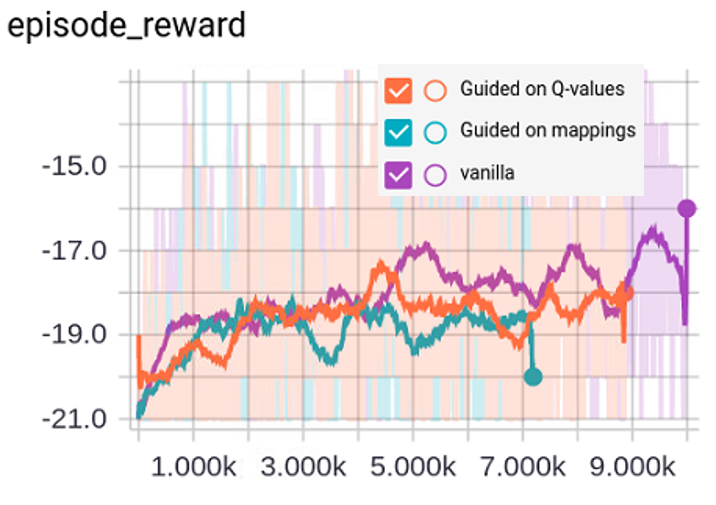
\includegraphics[scale=0.35,clip=true,trim = 0mm 0mm 0mm 0mm]{./fig/mimic_result_episode.png}
		\caption{Episode reward}
	\end{subfigure}%
	~ 
	\begin{subfigure}[t]{0.25\textwidth}
		\centering
		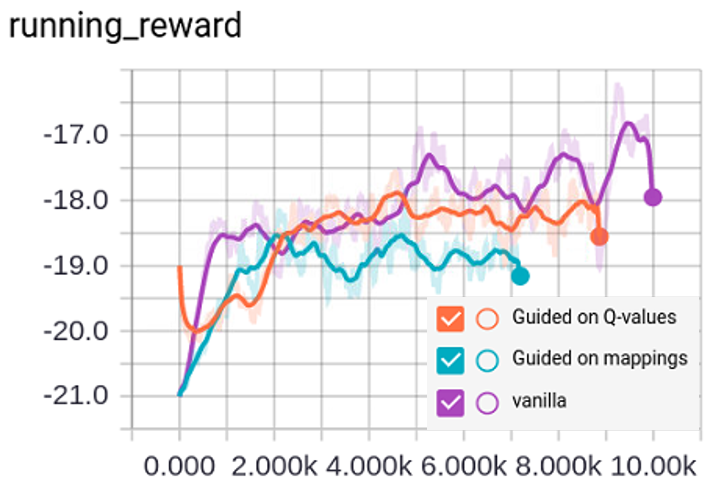
\includegraphics[scale=0.35,clip=true,trim = 0mm 0mm 0mm 0mm]{./fig/mimic_result_running.png}
		\caption{Running reward}
	\end{subfigure}
	\vspace{-1mm}
	\caption{The rewards of 10K epsiodes on three approaches: vanilla dueling Q-network, dueling Q-network guided on Q-values and dueling network guided on mapping of Q-values. Running reward is the smoothed accumulating rewards}
\label{fig:mimic_result}
	\vspace{-3mm}
\end{figure}






\section{Conclusion}
%!TEX root = main.tex

Our contribution in this project is summarized as follows:

First, we modify the dueling Q-network and policy gradient network which are implemented by others to play games on OpenAI gym.

Second, we investigate the effects of \textit{experience replay} and \textit{target Q-network} by conducting a several experiments. Experimental results show that \textit{experience replay} and \textit{target Q-network} can stabilize the training process.

Third, to investigate whether different agents can transfer knowledge between each other, we implement and use \textit{Knowledge Distillation } approach. The dueling Q-network is guided by policy gradient network during training. Through experiments we found that the dueling Q-network performs worse if it is directly guided on the Q-values. 
%
Maybe this could be solved by adding more fully-connected layers to project $Q(s,a;\theta_{Q})$ into another space to be guided by policy network.
%
Due to time limitation, we did not finish the experiments to verify our ideas.

%A3C
Fourth:

%-------------------------------------------------------------------------


% \section{Time Line}
% %!TEX root = main.tex


10/19-10/26: Review some related literatures about deep reinforcement learning-based games and related deep reinforcement learning methods. Figure out possible suitable methodologies and games to implement.

10/27-11/02: Review paper "Asynchronous Methods for Deep Reinforcement Learning". Learn to use OpenAI Gym, Keras software package.

11/09-11/16: Use Keras to define the deep q network. Write midterm paper.

11/16-11/23: OpenAI's gym library to interact with the game Learning Environment.

11/23-11/30: Use Tensorflow to optimization the network

12/01-12/13: Test the game. Write final report.





%-------------------------------------------------------------------------


{\small
\bibliographystyle{ieee}
\bibliography{egbib}
}

\end{document}
